\documentclass[11pt]{article}
\usepackage[a4paper, left=0.5in, right=0.5in, top=1in, bottom=1in]{geometry}
\usepackage{graphicx}
\usepackage{float}
%\usepackage{times}

\begin{document}
\title{CS296 Project : Crane Arm Simulation}
\author{Venkatesh Dupadda\\
		120050039\\
		120050039@iitb.ac.in \and 
        Siddhant Rajagopalan\\
		120100006\\
		rajgo94@gmail.com \and
		B.N.S Akshay Veer\\
		120050062\\
		akshayveer@iitb.ac.in
		\\}	
\date{\today} 
\maketitle

\section{Introduction}
Box2D is a 2D rigid body simulation library for games.It is a physics engine written in C++ for animation.As our course project we have designed a crane arm for lifing weights using Box2D.In this report we first discuss our original design and later we discuss our accomplished design and analysis of various parts of its code.
\section{Original Design}

\begin{figure}[ht!]
\centering
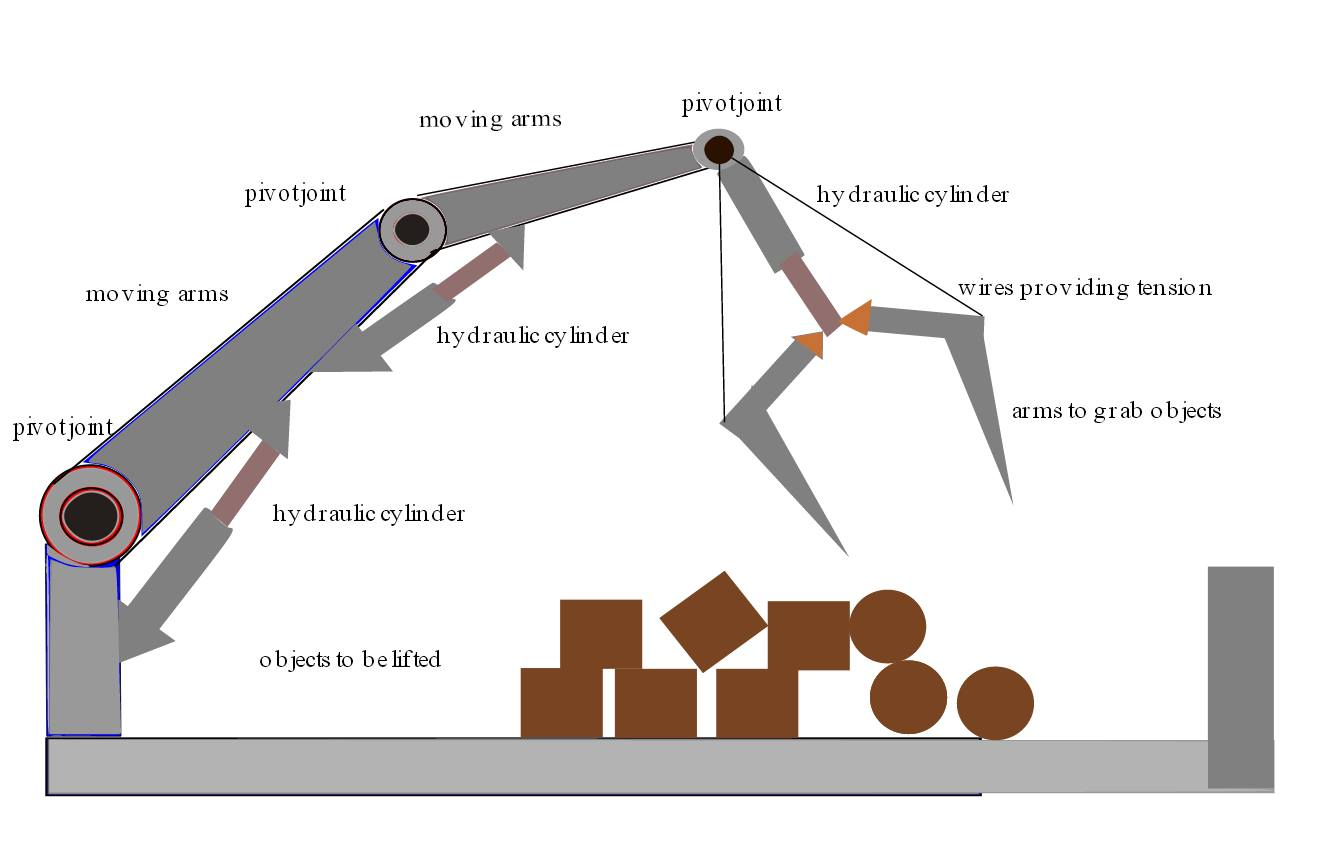
\includegraphics[height=11cm]{design.jpg}
\end{figure}

\subsection{Brief Description}
Hydraulic arm is used to lift and lower heavy objects.When we apply force on the hydraulic piston this moves the arms of the crane, which rotate on pivot joints and this causes force on the other piston which finally causes tension in rope.This tension in rope is used to move the arms required to hold or lower the objects.
\section{Final Design}

\begin{figure}[ht!]
\centering
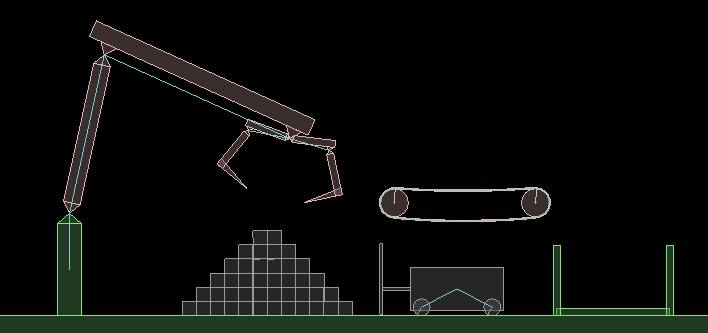
\includegraphics[height=9cm]{final.jpg}
\end{figure}

\subsection{Overall Description}
In this simulation we wanted to transfer the weights to container far away.This crane arm is controlled by the user.So we can lift the weights and place them on the conveyor belt.This converyor belt carries these weights to container.This is the overall idea of simulation.
\subsection{Description of Parts of Crane}
The crane is made up of both static and dynamic parts.The first arm is static and is attached to ground.Except the first arm all the remaining arms are dynamic.The second arm is connected to first arm and third arm by revoluting joints.Each revoluting joint has motor to control torque on that revoluting joint.The third arm is connected to second arm and to arms which are used to widen holder arms.Both the connecting joints are revolute joints.Finally both the holder arms are connected to arm which is used to widen these.

\subsection{Timing Analysis of Simulation}
\subsubsection{Average Step Time, Average Loop Time VS number of Iterations}
This is graph between Average Step Time, Average Loop Time versus number of iterations.
\\ \\ Average step time is independent of number of iterations because whatever may be number of iterations it takes same time for a step.So the Average step time versus number of iteration should be constant, since we have drawn histograms all of them should be of same height.The graph obtained also satisfies what we have observed.
\\ \\ Coming to the Average loop time versus this is nothing but (number of iterations * step time), since step time is independent of number of iterations we expect the graph to be linear, Indeed the graph is linear.Therefore our observations are correct.
\begin{figure}[ht!]
\centering
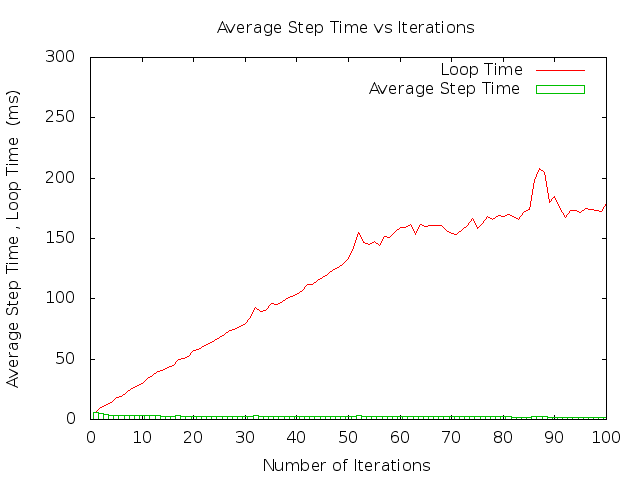
\includegraphics[height=8cm]{g23_plot01.png}
\end{figure}

\subsubsection{Average Step Time, Collision Resolution Time, Velocity Update Time, Position Update Time, and their sums VS Number of Iterations}
This is graph between the average of step time, average collision resolution time, average velocity update time, position update time, and their sum versus number of iterations.\\ \\
From the graph we can see that the averages of step time,collision resolution time, velocity update time, position update time are independent of n (with some disturbances when n is small). We can see that position update time and collision resolution time are nearly same.These time spent in updating positions and resolving collisons is less than velocity update time.So the simulation take more time in calculating velocities of bodies. We can observe that step size is more than sum of above times, from this we can infer that some time is spent on other parts.
\begin{figure}[H]
\centering
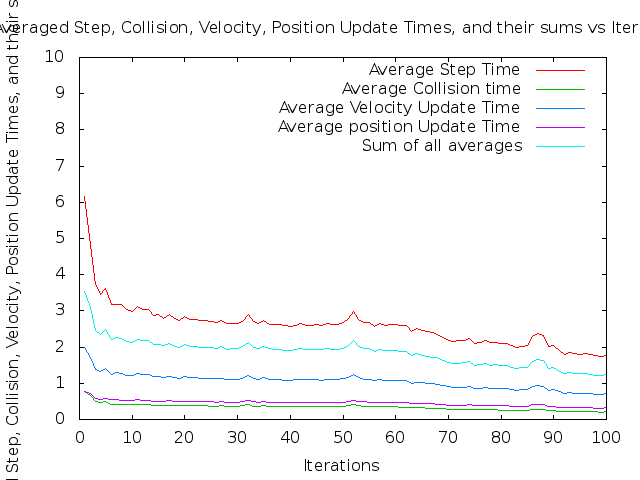
\includegraphics[height=8cm]{g23_plot02.png}
\end{figure}

\subsection{Errors in Reruns VS Number of Iterations}
This is graph between step time versus number of iterations along with error bars indicating variations in step time over all reruns.
From the graph we can observe that variation in step size over all reruns decreases, therefore all the error bars size decreases.
\begin{figure}[H]
\centering
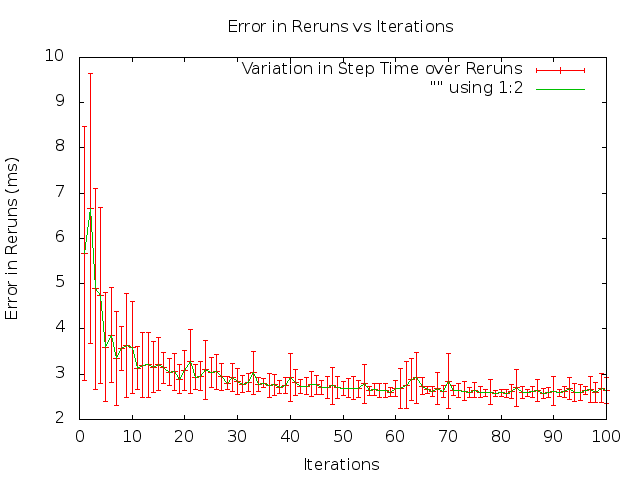
\includegraphics[height=8cm]{g23_plot03.png}
\end{figure}

\subsection{Best Fit Line for Average Step Time,15 Random ReRuns of Iterations VS Iterations}
This is graph of Best Fit Lines of Average Step Time, 15 ReRuns of a each iteration versus number of iterations.As we have observed in graph1 average step time is independent of number of iterations.So the expected best fit line should be nearly horizontal if n (number of iterations) is very large.From the obtained graph we can see that this is the case.
\begin{figure}[H]
\centering
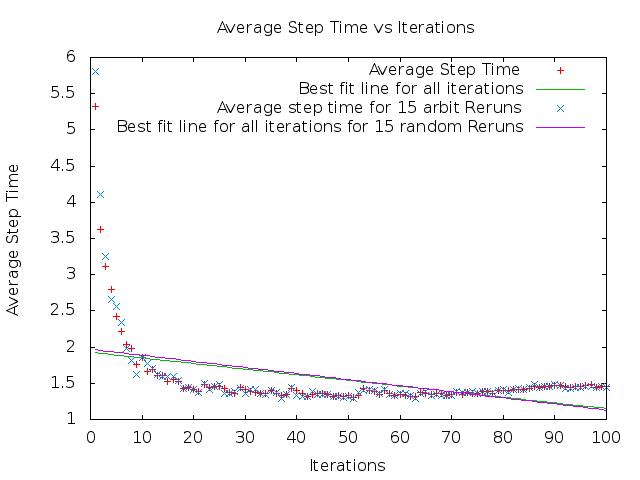
\includegraphics[height=8cm]{g23_plot04.png}
\end{figure}
\end{document}
